\documentclass[12pt, oneside, a4paper, chapter=TITLE,section=TITLE]{abntex2}

\usepackage{abntex2-ifrj} % pacote com customizações da classe abntex2 para uso no IFRJ-CVR

%Carregando alguns pacotes extras
\usepackage{float}
\usepackage{scalefnt}
\usepackage{supertabular,booktabs}
\usepackage{multirow} 

% ---
% Informações de dados para CAPA e FOLHA DE ROSTO
% ---
\titulo{Título do Trabalho}
\tipotrabalho{Relatório Técnico para Engenharia de Software} % colocar "pesquisa" ou "desenvolvimento tecnológico e inovação"
\autor{Alunos: [...], [...], [...] \\ Profa. Dra. Suéllen Martinelli }

\local{Capão Bonito}
\data{\today} % colocar a data de entrega ao CAP
\programa{Tecnologia em Sistemas Inteligentes}
% Preâmbulo 
\preambulo{\imprimirtipotrabalho\, desenvolvido pelos alunos [...], [...], [...] como parte dos critérios de avaliação da disciplina ministrada pela Profa. Dra. Suéllen Martinelli.
} % O preambulo deve conter o tipo do trabalho, o objetivo, o nome da instituição e a área de concentração

%\linhapesquisa{Otimização topológica} % colocar a linha de pesquisa à qual o projeto está vinculado, conforme o grupo de pesquisa do qual o pesquisador coordenador é integrante.

% --------------------------------
\makeindex % compila o índice remissivo (opcional)
% --------------------------------

% --------------------------------
% Início do documento
% --------------------------------
\begin{document}

% Retira espaço extra obsoleto entre as frases.
\frenchspacing

% --------------------------------
% ELEMENTOS PRÉ-TEXTUAIS
% --------------------------------
\pretextual
% ---
\imprimircapa % Capa
\imprimirfolhaderosto % Folha de rosto
% ---

% ---
% NOTA DA ABNT NBR 15287:2011, p. 4:
%  ``Se exigido pela entidade, apresentar os dados curriculares do autor em folha ou página distinta após a folha de rosto.''
% ---

% ---
% lista de ilustrações - Comente o código abaixo caso não tenha nenhuma imagem 
\pdfbookmark[0]{\listfigurename}{lof} \listoffigures*
\cleardoublepage
% ---

% ---
% lista de tabelas - Comente o código abaixo caso não tenha nenhuma tabela 
\pdfbookmark[0]{\listtablename}{lot}\listoftables*
\cleardoublepage
% ---

% ---
% inserir lista de quadros - Comente o código abaixo caso não tenha nenhum quadro 
\pdfbookmark[0]{\listofquadrosname}{loq} \listofquadros*
\cleardoublepage
% ---

% ---
% inserir lista de abreviaturas e siglas (opcional)
\begin{siglas}
  \item[ABNT] Associação Brasileira de Normas Técnicas
  \item[abnTeX] ABsurdas Normas para TeX
\end{siglas}
% ---


% ---
% inserir lista de símbolos
\begin{simbolos}
  \item[$ \Gamma $] Letra grega Gama
  \item[$ \Lambda $] Lambda
  \item[$ \zeta $] Letra grega minúscula zeta
  \item[$ \in $] Pertence
\end{simbolos}
% ---



% ---
% sumario
\pdfbookmark[0]{\contentsname}{toc}
\tableofcontents*
% \cleardoublepage
% ---


% --------------------------------
% ELEMENTOS TEXTUAIS
\textual
% --------------------------------

\chapter{Introdução}

Nesta área vcs escrevem o texto respectivo à introdução e apresentação do escopo do projeto. \cite{thinking2020design} Caso necessário citar referências, é possível usar o comando cite{} \cite{abntex2classe}.

\textbf{Versão prévia da introdução necessária na EP1.}

\chapter{Características do Projeto}

Nesta área vcs escrevem o texto respectivo aos principais dados e informações do projeto. Aqui nesta abertura vcs também vão \textbf{destacar qual foi o tema definido} pelo grupo, baseado nos primeiros dados e achados, bem como no que foi estipulado no Projeto Integrador.

\textbf{Obrigatório o preenchimento para EP1.}


\section{Problema e Objetivo}

Nesta seção vcs definem o problema, o objetivo geral e quais os objetivos específicos que permitem alcançar o objetivo geral.

\begin{itemize}
    \item gvhgffgfhfg
    \item cghgcbcvbc
\end{itemize}

\textbf{Conteúdo desta seção obrigatória na EP1.}


\section{Metodologia Utilizada: SCRUM}

Aqui vcs definem e explicam sobre o método usado no projeto (\textit{SCRUM}), com referências bibliográficas. Descrever sobre o funcionamento da \textbf{metodologia SCRUM} e como são definidos os principais \textbf{papéis} e \textbf{artefatos}.

\textbf{Conteúdo desta seção obrigatória na EP1.}



\begin{figure}[!ht]
\setlength{\itemsep}{0pt}
\setlength{\parskip}{0pt}
    \centering
    \caption{Legenda da Figura - Temos aqui um exemplo de imagem inserida em overleaf}
      
\includegraphics[width=0.5\columnwidth]{imagens/fatec.png}\\
      {Fonte: Da autora.}
      %\vspace{-0.6em}
      \label{fig:exemplo}
\end{figure}





\chapter{Entrega Parcial 1}

Cada capítulo nomeado como uma rodada parcial ou completa do SCRUM. \textbf{Aqui, vcs irão documentar até a conclusão do planejamento da primeira sprint no SCRUM.}

Dentro do capítulo, vcs escolhem como fazerem a documentação ou apresentação. Uma sugestão, é apresentarem e descreverem esses conteúdos em subseções com títulos respectivo à semana ou data da aula.

Neste texto, temos um exemplo de nota de rodapé, sobre o nome de uma base de dados chamada \textit{Engineering Village}\footnote{\url{ https://www.engineeringvillage.com/home.url}.}

\textbf{Conteúdo desta seção obrigatória para a EP1.}



\chapter{Entrega Parcial 2}

Cada capítulo nomeado como uma rodada parcial ou completa do SCRUM. \textbf{Aqui, vcs irão documentar a execução efetiva da primeira sprint no SCRUM.}

Dentro do capítulo, vcs escolhem como fazerem a documentação ou apresentação. Uma sugestão, é apresentarem e descreverem esses conteúdos em subseções com títulos respectivo à semana ou data da aula.

\textbf{Conteúdo desta seção obrigatória para a EP2.}



\chapter{Entrega Final}

Cada capítulo nomeado como uma rodada parcial ou completa do SCRUM. \textbf{Aqui, vcs irão documentar a segunda sprint completa efetuada dentro do SCRUM.}

Dentro do capítulo, vcs escolhem como fazerem a documentação ou apresentação. Uma sugestão, é apresentarem e descreverem esses conteúdos em subseções com títulos respectivo à semana ou data da aula.

\textbf{Conteúdo desta seção obrigatória para a Entrega Final.}



\chapter{Conclusão}

Elaborar uma conclusão ao projeto, sendo \textbf{preenchida apenas para a Entrega Final. }


\section{Limitações do Projeto}

Aqui o grupo vai descrever sobre as limitações do projeto, considerando limitações de tempo, de escopo, técnicas ou demais itens que tenham impactado na condução. \textbf{Preencher apenas para a Entrega Final.} 

\section{Lições Aprendidas}

Aqui o grupo vai descrever sobre as limitações do projeto, considerando limitações de tempo, de escopo, técnicas ou demais itens que tenham impactado na condução. \textbf{Preencher apenas para a Entrega Final.} 




% ---------------------------------
% ELEMENTOS PÓS-TEXTUAIS
% ---------------------------------
\phantompart
\postextual

% ---------------------------------
% Referências bibliográficas
% ---------------------------------
\bibliography{references}

% ---------------------------------
% Glossário
% ---------------------------------
%
% Consulte o manual da classe abntex2 para orientações sobre o glossário.
%
% \glossary

% ---------------------------------
% Apêndices  Elemento opcional
% ---------------------------------

\begin{apendicesenv} % Inicia os apêndices

\partapendices % Imprime uma página indicando o início dos apêndices

% ---------------------------------
\chapter{Exemplo 1: TCLE}
% ---------------------------------

\begin{figure}[!ht]
\setlength{\itemsep}{0pt}
\setlength{\parskip}{0pt}
    \centering
      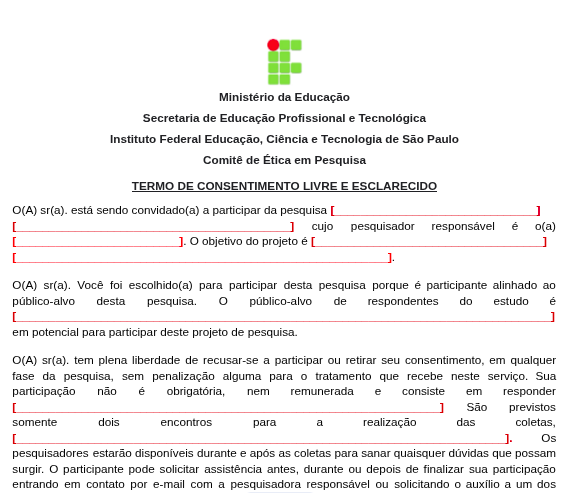
\includegraphics[width=0.7\columnwidth]{imagens/print_TCLE.png}\\
\end{figure}


% ---------------------------------
\chapter{Exemplo 2}
% ---------------------------------


\end{apendicesenv} % finaliza os apêndices
% ---


% ----------------------------------------------
% Anexos - Elemento opcional
% ----------------------------------------------
\begin{anexosenv} % Inicia os anexos

\partanexos % Imprime uma página indicando o início dos anexos

% ---
\chapter{Exemplo 1}
% ---
Pode-se anexar, ao final do projeto, material suplementar de sustentação à pesquisa: questionários, fotocópias, fotografias etc.


% ---
\chapter{Exemplo 2}
% ---



\end{anexosenv} % fim dos anexos

%------------------------------------------------------
% INDICE REMISSIVO - elemento opcional
%------------------------------------------------------
\phantompart
\printindex

\end{document}
